\documentclass[12pt, a4paper, oneside]{ctexart}
\usepackage{amsmath, amsthm, amssymb, bm, color, graphicx, geometry, mathrsfs,extarrows, braket, booktabs, array}
\usepackage[colorlinks,linkcolor=red,anchorcolor=blue,citecolor=blue,urlcolor=blue,menucolor=black]{hyperref}
\setmainfont{Times New Roman}  % 设置英文字体
\setsansfont{Calibri}
\setmonofont{Consolas}

\linespread{1.4}
%\geometry{left=2.54cm,right=2.54cm,top=3.18cm,bottom=3.18cm}
\geometry{left=1.84cm,right=1.84cm,top=2.18cm,bottom=2.18cm}
\newenvironment{problem}{\par\noindent\textbf{题目. }}{\bigskip\par}
\newenvironment{solution}{\par\noindent\textbf{解答. }}{\bigskip\par}
\newenvironment{note}{\par\noindent\textbf{注记. }}{\bigskip\par}

%%%% 图片相对路径 %%%%
\graphicspath{{figure/}} % 当前目录下的figure文件夹, {../figure/}则是父目录的figure文件夹

\everymath{\displaystyle} % 默认全部行间公式
\DeclareMathOperator*\uplim{\overline{lim}} % 定义上极限 \uplim_{}
\DeclareMathOperator*\lowlim{\underline{lim}} % 定义下极限 \lowlim_{}
\let\leq=\leqslant % 将全部leq变为leqslant
\let\geq=\geqslant % geq同理

% 一些宏定义
\def\bd{\boldsymbol}        % 加粗(向量) boldsymbol
\def\disp{\displaystyle}    % 使用行间公式 displaystyle(默认)
\def\tsty{\textstyle}       % 使用行内公式 textstyle
\def\sign{\text{sign}}      % sign function
\def\wtd{\widetilde}        % 宽波浪线 widetilde
\def\R{\mathbb{R}}          % Real number
\def\N{\mathbb{N}}          % Natural number
\def\Z{\mathbb{Z}}          % Integer number
\def\C{\mathbb{C}}          % Complex number
\def\d{\mathrm{d}}          % differential operator
\def\e{\mathrm{e}}          % Euler's number
\def\i{\mathrm{i}}          % imaginary number
\def\re{\mathrm{Re}}        % Real part
\def\im{\mathrm{Im}}        % Imaginary part
\def\res{\mathrm{Res}}      % Residue
\def\L{\mathcal{L}}         % Loss function
\def\wdh{\widehat}          % 宽帽子 widehat
\def\ol{\overline}          % 上横线 overline
\def\ul{\underline}         % 下横线 underline
\def\add{\vspace{1ex}}      % 增加行间距
\def\del{\vspace{-3.5ex}}   % 减少行间距

% 基本信息
\newcommand{\RQ}{\today} % 日期
\newcommand{\km}{实变函数} % 科目
\newcommand{\bj}{强基数学002} % 班级
\newcommand{\xm}{吴天阳} % 姓名
\newcommand{\xh}{2204210460} % 学号

\begin{document}

% 正文部分
\section*{基本概念}
\textbf{最优化问题的数学模型的一般形式(优化模型):}(第七章又重新定义了一遍, 只是符号有所不同, 这里定义为极小化问题, 极大化问题可以转化为极小化问题)
\begin{equation*}
    \left\{\begin{aligned}
        \min &\ \ f(x)\\
        \text{s.t.}&\ \ c_i(x) = 0,\ i=1,2,\cdots, m,\\
        &\ c_i(x)\geq 0,\ i=m+1,\cdots, p,
    \end{aligned}\right.
\end{equation*}
其中$x=(x_1,x_2,\cdots, x_n)^T\in\R^n$, $f:\R^n\to\R^1$, $c_i = \R^n\to \R^1(i=1,2,\cdots, p)$为连续函数, 通常还要求连续可微. $x$称为\textbf{决策变量}, $f(x)$为\textbf{目标函数}, $c_i(x),i=1,2,\cdots, p$为\textbf{约束函数(约束条件)}, $c_i(x) = 0,\ i=1,2,\cdots, m$为\textbf{等式约束}, $c_i(x)\geq 0,\ i=m+1,\cdots, p$为\textbf{不等式约束}, 并记等式约束指标集为$E=\{1,2,\cdots, m\}$, 不等式约束指标集为$I=\{m+1,\cdots, p\}$.

\textbf{可行点}: 若点$x\in\R^n$满足优化模型中的所有约束条件, 则称$x$为\textbf{可行点}.

\textbf{可行域}: 全体可行点所成之集称为\textbf{可行域}, 即
\begin{equation*}
    \mathcal{F} = \{x:c_i(x) = 0,\ i=1,2,\cdots, m,\ c_i(x)\geq 0, i=m+1,\cdots, p\}.
\end{equation*}

\textbf{有效约束(起作用约束)}: 可行点$\bar{x}\in\mathcal{F}$, 若$c_i(\bar{x}) = 0$, 则称不等式约束$c_i(x)\geq 0$在点$\bar{x}$是\textbf{有效约束}, 并称可行点$\bar{x}$位于约束$c_i(x)\geq 0$的边界.

\textbf{有效约束集}: 记$I(x) = \{i:c_i(x) = 0,\ i\in I\}$, 对任何$x\in\R^n$, 我们称集合
\begin{equation*}
    A(x) = E\cup I(x)
\end{equation*}
是在$x$点处的\textbf{有效约束指标集(或积极约束指标集)}, 简称\textbf{有效约束集或有效集}.

\textbf{可行方向}: 设$x^*\in \mathcal{F}$, $0\neq d\in\R^n$, 若存在$\delta > 0$使得
\begin{equation*}
    x^* + \alpha d\in \mathcal{F},\quad \forall \alpha\in[0,\delta],
\end{equation*}
则称$d$是$\mathcal{F}$在$x^*$处的\textbf{可行方向}. $\mathcal{F}$在$x^*$处的全体可行方向所成之集记为$\mathcal{FD}(x^*, \mathcal{F})$.

\textbf{下降方向}: 设$f(x)$为$\R^n$上的连续函数, 点$\bar{x}\in\R^n$, 若对于方向$s\in\R^n$存在$\delta >0$使得下式成立
\begin{equation*}
    f(\bar{x}+\alpha s) < f(\bar{x}),\quad\forall \alpha\in(0,\delta),
\end{equation*}
则称$s$为$f(x)$在$\bar{x}$处的一个\textbf{下降方向}, 将点$\bar{x}$处的所有下降方向所成之集记为$\mathcal{D}(\bar{x})$.

\textbf{无效约束(不起作用约束)}: 可行点$\bar{x}\in\mathcal{F}$, 若$c_i(\bar{x}) > 0$, 则称不等式约束$c_i(x)\geq 0$在点$\bar{x}$是\textbf{无效约束}, 并称可行点$\bar{x}$位于约束$c_i(x)\geq 0$的内部.

\textbf{全局(或总体)最优解(极小点)}: 可行点$x^*\in \mathcal{F}$称为优化模型的\textbf{全局最优解}, 当且仅当
\begin{equation*}
    f(x^*)\leq f(x),\quad \forall x\in \mathcal{F}.
\end{equation*}

\textbf{严格全局(或总体)最优解(极小点)}: 可行点$x^*\in \mathcal{F}$称为优化模型的\textbf{严格全局最优解}, 当且仅当
\begin{equation*}
    f(x^*)< f(x),\quad \forall x\in \mathcal{F},\ x\neq x^*.
\end{equation*}

\textbf{局部最优解(极小点)}: 可行点$x^*\in \mathcal{F}$称为优化模型的\textbf{局部最优解}, 当且仅当, 存在$x^*$的一个邻域
\begin{equation*}
    \mathcal{N}(x^*) = \{x:||x-x^*|| \leq \delta\}
\end{equation*}
使得下式成立
\begin{equation*}
    f(x^*)\leq f(x),\quad \forall x\in\mathcal{N}(x^*)\cap\mathcal{F}.
\end{equation*}
同理也可以定义严格局部最优解.

\textbf{严格局部最优解(极小点)}: 可行点$x^*\in \mathcal{F}$称为优化模型的\textbf{严格局部最优解}, 当且仅当, 存在$x^*$的一个邻域
\begin{equation*}
    \mathcal{N}(x^*) = \{x:||x-x^*|| \leq \delta\}
\end{equation*}
使得下式成立
\begin{equation*}
    f(x^*)< f(x),\quad \forall x\in\mathcal{N}(x^*)\cap\mathcal{F},\ x\neq x^*.
\end{equation*}

\textbf{凸集}: 集合$D\subset \R^n$称为\textbf{凸集}, 当且仅当, 对于任意$x,y\in D$有
\begin{equation*}
    \lambda x+(1-\lambda)y\in D,\quad\forall \lambda\in[0,1].
\end{equation*}
即连接$x, y$的直线段上的所有点均在集合$D$内.

\textbf{凸函数}: 设函数$f(x)$在凸集$D$上有定义, 如果对于任意$x, y\in D$有
\begin{equation*}
    f(\lambda x+(1-\lambda)y)\leq \lambda f(x)+(1-\lambda)f(y),\quad \forall \lambda\in[0,1],
\end{equation*}
则称$f(x)$是凸集$D$上的\textbf{凸函数}.

\textbf{严格凸函数}: 设函数$f(x)$在凸集$D$上有定义, 如果对于任意$x, y\in D,\ x\neq y$有
\begin{equation*}
    f(\lambda x+(1-\lambda)y)< \lambda f(x)+(1-\lambda)f(y),\quad \forall \lambda\in(0,1),
\end{equation*}
则称$f(x)$是凸集$D$上的\textbf{严格凸函数}.

\textbf{凸规划问题}: 可行域$\mathcal{F}$是凸集, 目标函数$f(x)$是凸函数的最优化问题称为\textbf{凸规划问题}. (可以证明, 凸规划问题的局部最优解必是全局最优解)

\textbf{判断凸函数方法}: 设$f(x)$为非空开凸集$D\subset \R^n$上的二阶可微函数, 则

(1) $f(x)$的Hesse矩阵$\nabla^2 f(x)$在$D$上\textbf{半正定}(所有主子式均$\geq 0$)$\iff$$f(x)$是$D$上的\textbf{凸函数}.

(2) $f(x)$的Hesse矩阵$\nabla^2 f(x)$在$D$上\textbf{正定}(顺序主子式均$ > 0$)$\Rightarrow$$f(x)$是$D$上的\textbf{严格凸函数}.

\textbf{最优性条件}: 最优化问题的最优解(局部的或者全局的)所必须满足的条件.

\textbf{KKT点}: 利用迭代的方法产生一个逐步改善的序列$\{x^{(k)}\}$, 在$\{x^{(k)}\}$为\textbf{有限}点列时, 它最后一个点是\textbf{KKT点}; 当$\{x^{(k)}\}$是\textbf{无限点列}时, 其任意一个聚点为\textbf{KKT点}.

\textbf{最优化方法的基本迭代格式}:
\begin{enumerate}
    \item 给出初始点$x^{(0)}$, 令$k:=0$; (初始化)

    \item 如果$x^{(k)}$满足对最优解估计的终止条件, 停止迭代; (结束条件)

    \item 确定一个改善$x^{(k)}$的修正量$s^{(k)}$; (计算)

    \item 令$x^{(k+1)} = x^{(k)} + s^{(k)},\ k:=k+1$, 转到第2步. (更新)
\end{enumerate}


\textbf{算法(方法)的收敛性}: 一个算法是收敛的, 当且仅当, 算法产生的序列$\{x^{(k)}\}$满足
\begin{equation*}
    \lim_{k\to\infty}||x^{(k)}-x^*|| = 0,
\end{equation*}
其中$x^*$为该问题的KKT点, 即该序列$\{x^{(k)}\}$收敛.

\textbf{全局收敛(总体收敛)}: 如果一个算法对于任意给定的初始点都能能够收敛, 则称该算法\textbf{全局收敛}.

\textbf{局部收敛}: 如果一个算法只有当初始点接近或充分接近最优解时才具有收敛性, 则称该算法\textbf{局部收敛}.

\textbf{收敛速度}: 设向量序列$\{x^{(k)}\}\subset \R^n$收敛于$x^*$, 定义误差序列
\begin{equation*}
    e_k = x^{(k)} - x^*.
\end{equation*}
若存在正常数$C$和$r$使得下式成立
\begin{equation*}
    \lim_{k\to\infty}\frac{||x^{(k+1)}-x^*||}{||x^{(k)}-x^*||^r}=\lim_{k\to\infty}\frac{||e_{k+1}||}{||e_k||^r} = C,
\end{equation*}
则称序列$\{x^{(k)}\}$ $\bd{r}$\textbf{阶}收敛于$x^*$(以$C$为因子, 有时也称$C$为\textbf{收敛速度的值}).

当$r=1,\ 0 < C < 1$时称为\textbf{线性收敛}, $r=2$时称为\textbf{二次收敛}, $r > 1$时称为\textbf{超线性收敛}.

\textbf{精确线性搜索的无约束最优化算法的一般形式}:
\begin{enumerate}
    \item 给出初始点$x_0\in\R^n$, $\varepsilon \geq 0$, 令$k:=0$.

    \item 计算$\nabla f(x_k)$, 若$||\nabla f(x_k)||\leq \varepsilon$, 停止迭代.

    \item 计算下降方向$d_k$, 计算步长因子$\alpha_k$, 使得
    \begin{equation*}
        f(x_k+\alpha_kd_k) = \min_{\alpha \geq 0} f(x_k+\alpha d_k).
    \end{equation*}

    \item 令$x_{k+1} = x_k+\alpha_kd_k$, $k:=k+1$, 转到第2步.
\end{enumerate}

\section*{5种无约束最优化方法}

\textbf{最速下降法}: 设目标函数$f(x)$在$x_k$附近连续可微, 且$g_k:= \nabla f(x_k)\neq 0$.
\begin{enumerate}
    \item 给出初始点$x_0\in\R^n$, $\varepsilon\geq 0$, 令$k:= 0$.
    \item 计算$d_k = -g_k$; 若$||g_k|| \leq \varepsilon$, 停止迭代.
    \item 计算步长因子$\alpha_k$, 使得
    \begin{equation*}
        f(x_k+\alpha_kd_k) = \min_{\alpha \geq 0} f(x_k+\alpha d_k).
    \end{equation*}
    \item 令$x_{k+1} = x_k+\alpha_kd_k$, $k = k+1$, 转到第2步.
\end{enumerate}

\textbf{带步长因子的牛顿法}: 设$f(x)$二次连续可微, $x_k \in \R^n$, 令$G_k:= \nabla^2 f(x_k),\ g_k:= \nabla f(x_k)$.
\begin{enumerate}
    \item 给出初始点$x_0$, $\varepsilon \geq 0$, 令$k:=0$.
    \item 计算$g_k$. 若$||g_k|| \leq \varepsilon$, 停止迭代.
    \item 解方程组$G_kd = -g_k$得$d_k$为牛顿方向, 计算步长因子$\alpha_k$, 使得
    \begin{equation*}
        f(x_k+\alpha_kd_k) = \min_{\alpha \geq 0} f(x_k+\alpha d_k).
    \end{equation*}
    \item 令$x_{k+1} = x_k + \alpha_k d_k$, $k:= k+1$, 转到第2步.
\end{enumerate}


牛顿法具有\textbf{2阶}收敛速度.

\textbf{向量的共轭}: 设$G$是$n\times n$对称正定矩阵, $d_1, d_2$为$n$为非零向量, 若
\begin{equation*}
    d_1^T Gd_2 = 0,
\end{equation*}
则称向量$d_1$和$d_2$是$G$-共轭的, 简称\textbf{共轭的}.

$d_1, d_2,\cdots, d_m$为一组$n$为非零向量, 若
\begin{equation*}
    d_i^T Gd_j = 0,\quad(i\neq j),
\end{equation*}
则称向量$d_1, d_2, \cdots, d_m$是$G$-共轭的, 简称\textbf{共轭的}.

\textbf{一般共轭方向法}: 
\begin{enumerate}
    \item 给出初始点$x_0$, $\varepsilon\geq 0$, 令$k:=0$.
    
    计算$g_0 = \nabla f(x_0)$和初始下降方向$d_0$, 使得$d_0^Tg_0 < 0$.
    \item 计算$g_k$. 如果$||g_k||\leq \varepsilon$, 停止迭代.
    \item 计算步长因子$\alpha_k$, 使得
    \begin{equation*}
        f(x_k+\alpha_kd_k) = \min_{\alpha \geq 0} f(x_k+\alpha d_k).
    \end{equation*}
    \item 采用某种共轭方向法计算$d_{k+1}$使得
    \begin{equation*}
        d_{k+1}^TGd_j = 0,\ j=0,1,\cdots, k.
    \end{equation*}
    令$x_{k+1} = x_k + \alpha_k d_k$, $k:=k+1$, 转到第2步. 
\end{enumerate}

\textbf{二次终止性}: 对于正定二次函数, 算法是有限步终止的. (可以证明若搜索方向是相互共轭的, 则算法具有二次终止性, \textbf{共轭梯度法和拟牛顿法}都就具有\textbf{二次终止性})

\textbf{拟牛顿法}: $B_k$为牛顿法迭代中的Hesse矩阵$G_k$的近似值, 通常取$B_0 = E_n$单位阵.
\begin{enumerate}
    \item 给出初始点$x_0\in \R^n$, $B_0\in \R^{n\times n}$, $\varepsilon\geq 0$, $k:=0$.
    \item 计算$g_k = \nabla f(x_k)$. 如果$||g_k|| \leq \varepsilon$, 停止迭代.
    \item 解方程组$B_kd = -g_k$得到搜索方向$d_k$, 计算步长因子$\alpha_k$, 使得
    \begin{equation*}
        f(x_k+\alpha_kd_k) = \min_{\alpha \geq 0} f(x_k+\alpha d_k).
    \end{equation*}
    \item 令$x_{k+1} = x_k + \alpha_k d_k$. 校正$B_k$产生$B_{k+1}$, 使得拟牛顿条件
    \begin{equation*}
        B_k(x_{k+1}-x_k) = g_{k+1} - g_k,
    \end{equation*}
    成立, 其中$g_{k+1} = \nabla f(x_{k+1})$. 令$k:=k+1$, 转到第2步.
\end{enumerate}

\textbf{最小二乘问题}:
\begin{equation}\label{two}
    \min_{x\in\R^n}\quad f(x) = \frac{1}{2}||r(x)||_2^2 = \frac{1}{2}\sum_{i=1}^m[r_i(x)]^2,\quad m\geq n.
\end{equation}
其中$r(x) = (r_1(x), r_2(x),\cdots, r_m(x))^T$, $r_i(x)\ (i=1,2,\cdots, m)$称为\textbf{残量函数}, 有无$\frac{1}{2}$对最优解没有影响. 当$r_i(x)$为线性函数时, 称(\ref{two})为\textbf{线性最小二乘问题}; 当$r_i(x)$为非线性函数时, 称(\ref{two})为\textbf{非线性最小二乘问题}.

\textbf{Gauss-Newton法求解非线性最小二乘问题}: 记向量函数$r(x)$的$m\times n$阶Jacobian矩阵为
\begin{equation*}
    A(x) = \nabla r(x) = [\nabla r_1(x),\cdots,\nabla r_m(x)]^T = \left[\begin{matrix}
        \frac{\partial r_1}{\partial x_1}(x) & \frac{\partial r_1}{\partial x_2}(x) & \cdots & \frac{\partial r_1}{\partial x_n}(x) \add\\
        \frac{\partial r_2}{\partial x_1}(x) & \frac{\partial r_2}{\partial x_2}(x) & \cdots & \frac{\partial r_2}{\partial x_n}(x) \add\\
        \vdots&\vdots&\ddots&\vdots\add\\
        \frac{\partial r_m}{\partial x_1}(x) & \frac{\partial r_m}{\partial x_2}(x) & \cdots & \frac{\partial r_m}{\partial x_n}(x)
    \end{matrix}\right]
\end{equation*}
记$A_k = A(x_k),\ r_k = r(x_k)$, 则Gauss-Newton法如下
\begin{enumerate}
    \item 给定初始值$x_k$, $\varepsilon\geq 0$, 令$k:=0$.
    \item 计算$g_k = \nabla f(x_k)$. 若$||g_k||\leq \varepsilon$, 停止迭代.
    \item 解方程组$A_k^TA_k\delta = -A_k^Tr_k$得到搜索方向$\delta_k$.
    \item 令$x_{k+1} = x_k + \delta_k$, $k:=k+1$, 转到第2步.
\end{enumerate}

\section*{KKT条件}
\textbf{KKT定理}: 设$f(x), c_i(x)\ (i=1,2,\cdots, p)$在$x^*$的邻域内一阶连续可微, 约束规范条件(应该不是重点)
\begin{equation*}
    \mathcal{SFD}(x^*, \mathcal{F}) = \mathcal{LFD}(x^*, \mathcal{F})
\end{equation*}
成立, 则存在$\lambda_i^*\ (i=1,2,\cdots, m)$使得(下面五个条件就是\textbf{KKT条件})
\begin{align}
    &\nabla f(x^*) = \sum_{i=1}^m \lambda_i^*\nabla c_i(x^*),&\text{驻点条件}\label{lag}\\
    &c_i(x^*) = 0,\quad i\in E,&\text{等式约束条件}\nonumber\\
    &c_i(x^*)\geq 0, i\in I,&\text{不等式约束条件}\nonumber\\
    &\lambda_i^*\geq 0,\quad i\in I,&\text{非负乘子条件}\nonumber\\
    &\lambda_i^*c_i(x^*) = 0,\quad i\in I.&\text{互补松弛条件}\nonumber
\end{align}
若记\textbf{Lagrange函数}$L(x,\lambda^*) = f(x) - \sum_{i=1}^m\lambda_i^*c_i(x)$, 则KKT条件中第一个条件(即(\ref{lag})式)可以视为
\begin{equation*}
    \nabla_xL(x^*, \lambda^*) = \frac{\partial L}{\partial x}(x^*) = \left[\begin{matrix}
        \frac{\partial L}{\partial x_1}(x^*)&\cdots&\frac{\partial L}{\partial x_n}(x^*)
    \end{matrix}\right]^T = \bd{0}
\end{equation*}
\textbf{注意}: 使用上述KKT条件, 必须满足为极小化问题, 且\textbf{不等式约束为$\geq 0$的形式}.

\section*{二次罚函数和内点障碍法}
只需会构造即可.

\textbf{二次罚函数}: 关于优化模型我们定义二次罚函数$Q(x;\mu)$如下
\begin{equation*}
 Q(x:\mu):= f(x) +\frac{1}{2\mu}\sum_{i\in E}c_i^2(x)+\frac{1}{2\mu}\sum_{i\in I}([c_i(x)]^-)^2   
\end{equation*}
其中$[c_i(x)]^-:=\min\{c_i(x), 0\}, (i\in I)$, $\frac{1}{2\mu}$称为罚系数.\add

当罚系数$\to\infty$时, $Q(x;\mu)$的极小值趋近优化模型的极小值.

\textbf{内点障碍法}: 考虑不等式约束最优化问题
\begin{equation*}
    \left\{\begin{aligned}
        \min &\ \ f(x)\\
        \text{s.t.}&\ c_i(x)\geq 0,\ i=I.
    \end{aligned}\right.
\end{equation*}
两种常用的障碍函数:

\textbf{对数障碍函数}: 
\begin{equation*}
    P(x;\mu) = f(x)-\mu\sum_{i\in I}\log c_i(x).
\end{equation*}
\textbf{分数障碍函数}:
\begin{equation*}
    P(x;\mu) = f(x)-\mu\sum_{i\in I}\frac{1}{[c_i(x)]^+}.
\end{equation*}
其中$[c_i(x)]^+ = \max\{0,c_i(x)\}$.

当$\mu\to 0$时, $P(x;\mu)$的极小值趋近优化模型的极小值. 

内点障碍法的优势在于, $P(x,\mu)$每一步所求出的的极小值, 一定符合优化模型的所有不等式约束条件, 而罚函数方法并不能保证.

% 下面给一些功能的写法
\iffalse
% 图片模板
\centerline{
    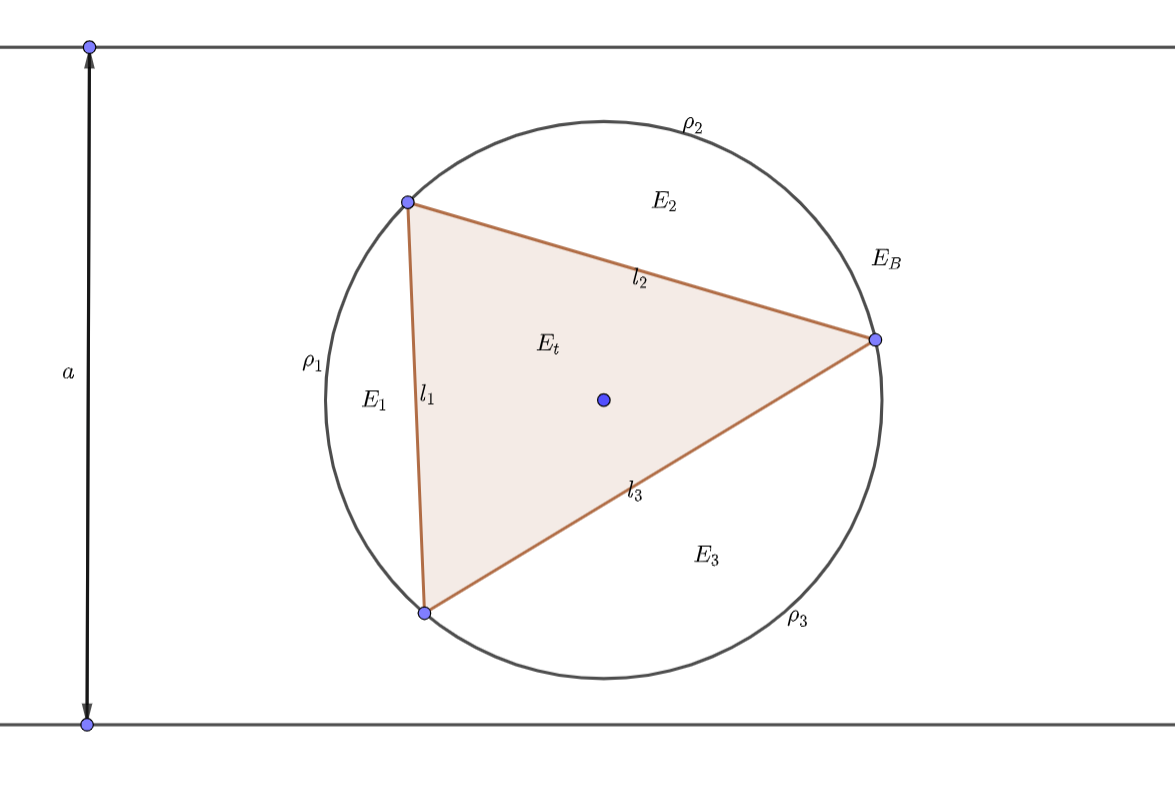
\includegraphics[width=0.8\textwidth]{figure.png}
}
% 表格模板
\renewcommand\arraystretch{0.8} % 设置表格高度为原来的0.8倍
\begin{table}[!htbp] % table标准
    \centering % 表格居中
    \begin{tabular}{p{1cm}<{\centering}p{1cm}<{\centering}p{3cm}<{\centering}p{5cm}<{\centering}} % 设置表格宽度
    %\begin{tabular}{cccc}
        \toprule
        $x_i$ & $f[x_1]$ & $f[x_i,x_{i+1}]$ & $f[x_i,x_{i+1},x_{i+2}]$ \\
        \midrule
        $x_0$ & $f(x_0)$ &                  &                          \\
        $x_0$ & $f(x_0)$ & $f'(x_0)$        &                          \\
        $x_0$ & $f(x_1)$ & $\frac{f(x_1)-f(x_0)}{x_1-x_0}$ & $\frac{f(x_1)-f(x_0)}{(x_1-x_0)^2}-\frac{f'(x_0)}{x_1-x_0}$\\
        \bottomrule
    \end{tabular}
\end{table}

\def\Log{\text{Log}} % 一个简单的宏定义
$\Log$ % 调用方法
\fi

\end{document}